\documentclass{article}
\usepackage[spanish]{babel}   
\usepackage[numbers,sort&compress]{natbib}
\usepackage{float}
\usepackage{listings}
\usepackage{graphicx} 	% Nos permite importar imagenes 
\usepackage{subfigure}
\usepackage[left=3cm,right=3cm,top=3cm,bottom=3cm]{geometry}

%-------------------------- Por si se romple la URL --------------------------
\usepackage[hyphens]{url}
\usepackage[hidelinks]{hyperref}
\hypersetup{breaklinks=true}	
\urlstyle{same}
\usepackage{cite}
%-------------------------- Por si se romple la URL --------------------------

\title{Reporte Tarea 6}
\author{Victor Alejandro Oviedo Martínez}



\begin{document}
\maketitle
\hrule

\section{Introduccón}\label{intro}
Para esta séptima tarea\citep{DRA.P7} se ha estudiado el tema búsqueda local, en la cual se presenta una función $f(x)$ la cual buscamos encontrar el valor mas pequeño. Tomando en cuenta que tendremos una posición inicial $x$, modificaremos esta posición con $\Delta x > 0$ y con esto se calcula $f(x \pm \Delta x)$ para determinar cuál es la menor y convertir esta en nuestra nueva $x$. Este procedimiento se repite la cantidad de veces que sean necesarias para encontrar el valor mínimo de toda la función.




\section{Desarrollo}

Para esta séptima tarea se ha planteado el siguiente problema: La tarea se trata de maximizar algún variante de la función bidimensional ejemplo $g(x,y)$,  con restricciones $ -3\leq x,y \leq 3$, con la misma técnica del ejemplo unidimensional. La posición actual es un par y se ocupan dos movimientos aleatorios, $\Delta x$ y $\Delta y$ , cuyas combinaciones posibles proveen ocho posiciones vecino, de los cuales aquella que logra el mayor valor para es seleccionado.Crear una visualización animada de cómo proceden réplicas simultáneas de la búsqueda encima de una gráfica de proyección plana.\\

Para el desarrollo de esta tarea se han utilizado los códigos ejemplo proporcionado por \citet{DRA.Code},\citep{DRA.Code2}, el cual tiene el propósito de: poder observar la visualización de la búsqueda local en un función de dos dimensiones \citep{DRA.Code2}, y observar la visualización con múltiples puntos de la búsqueda local en una función de dos dimensiones \citep{DRA.Code}. Estos dos códigos será tomados como base para entregar las características de esta tarea.\\

Para el desarrollo de esta tarea se iniciado observando \citep{DRA.Code} y \citep{DRA.Code2}, con esto se reflexionó a iniciar primero con una versión sencilla del programa final, en el cual este tendría como objetivo encontrar el máximo de la búsqueda local con un solo punto, para después intentar realizar lo mismo, pero esta vez con los quince puntos pedidos.\\

Por lo tanto, se ha iniciado con la definición de la función a evaluar \ref{eq:e1}, y agregar variables que son necesarias para graficar la función con una vista superior.\\

\begin{equation}
\label{eq:e1}
 g(x,y)= \frac{(x + 0.25)^4 - 30 * x^2 - 20 * x + (y + 0.25)^4 - 30 * y^2 - 20 * y)}{50} 
\end{equation}

\begin{figure}[H]
\begin{center}
	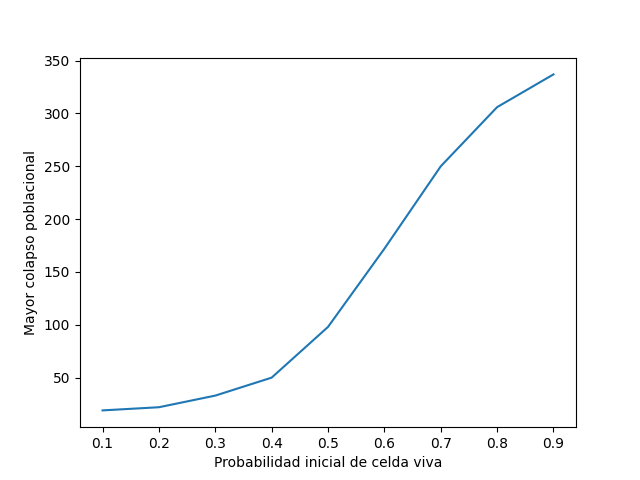
\includegraphics[height=3.5in]{/Users/victor/Desktop/Figure_1.png}
	\caption{ $g(x,y)$ con $-3\leq x,y \leq 3$.}
	\label{fig:cuadro.1}
\end{center}
\end{figure}

\begin{lstlisting}[language=Python]

def g(x, y):
    return ((x + 0.25)**4 - 30 * x**2 - 20 * x + (y + 0.25)**4 - 30 * y**2 - 20 * y)/50



tmax = 100
digitos = floor(log(tmax, 10)) + 1
low = -3
high = 3
step = 0.1
p = np.arange(low, high, step)
n = len(p)
z = np.zeros((n, n), dtype=float)
for i in range(n):
    x = p[i]
    for j in range(n):
        y = p[n - j - 1] # voltear
        z[i, j] = g(x, y)
 \end{lstlisting}
 
 Después, se procede a generar las condiciones iniciales 

\begin{lstlisting}[language=Python]
X = uniform(low, high)
Y = uniform(low, high)
curr = [X,Y]
best = curr
paso = 0.3
 \end{lstlisting}


Una vez teniendo las condiciones iniciales, incluimos un ciclo $for$ con el fin de repetir los movimientos de nuestro punto y graficar cada movimiento. Dentro del ciclo $for$ se inicia obteniendo $\Delta x$ y $\Delta y$, y en base a este se genera posibles movimiento los cuales son evaluados para determinar cuál de todos ellos se acerca más al punto más alto. La variable \texttt{best} será la encargada de guardar el valor mas alto de todas las repeticiones.


\begin{lstlisting}[language=Python]
for tiempo in range(tmax):

    deltaX = uniform(0, paso)
    deltaY = uniform(0, paso)
    leftX = curr[0] - deltaX
    rightX = curr[0] + deltaX
    leftY = curr[1] - deltaY
    rightY = curr[1] + deltaY

    RXRY = g(rightX,rightY)
    LXRY = g(leftX,rightY)
    RXLY = g(rightX,leftY)
    LXLY = g(leftX,leftY)

    if RXRY > LXRY and RXRY > RXLY and RXRY > LXLY:
        curr = [rightX,rightY]
    if LXRY > RXRY and LXRY > RXLY and LXRY > LXLY:
        curr = [leftX,rightY]
    if RXLY > RXRY and RXLY > LXLY and RXLY > LXLY:
        curr = [rightX,leftY]
    if LXLY > RXRY and LXLY > LXRY and LXLY > RXLY:
        curr = [leftX,leftY]

    if g(curr[0],curr[1]) > g(best[0],best[1]):
        best = curr



    t = range(0, n, 5)
    l = ['{:.1f}'.format(low + i * step) for i in t]
    fig, ax = plt.subplots(figsize=(6, 5), ncols=1)
    pos = ax.imshow(z)
    ax.scatter(interX(best[0]), interY(best[1]), marker = 'v', color = '#0000ff')
    ax.scatter(interX(curr[0]), interY(curr[1]), marker = '1', color = 'red')
    plt.xticks(t, l)
    plt.yticks(t, l[::-1]) # arriba-abajo
    fig.colorbar(pos, ax=ax)
    plt.title('Paso {:d}'.format(tiempo + 1))
    fig.savefig('p7p_t' + format(tiempo, '0{:d}'.format(digitos)) + '.png')
    plt.close()
 \end{lstlisting}
 
 Por último, se grafican todos los resultados de cada paso. Dado el método utilizado para graficar la función se ha tenido que crear dos funciones $interX$ y $interY$, con el fin de interpolar los valores de la gráfica para que los valores coincidan con las etiquetas. 
 
\begin{figure}[H]
\centering
\subfigure[Paso 1]{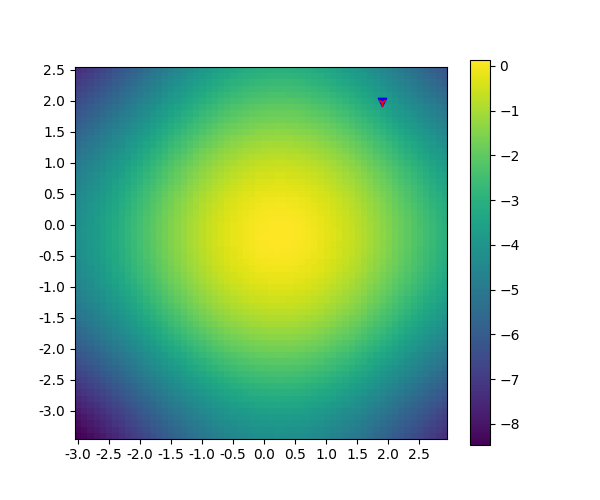
\includegraphics[width=60mm]{/Users/victor/Desktop/p7p_t000.png}}
\subfigure[Paso 50]{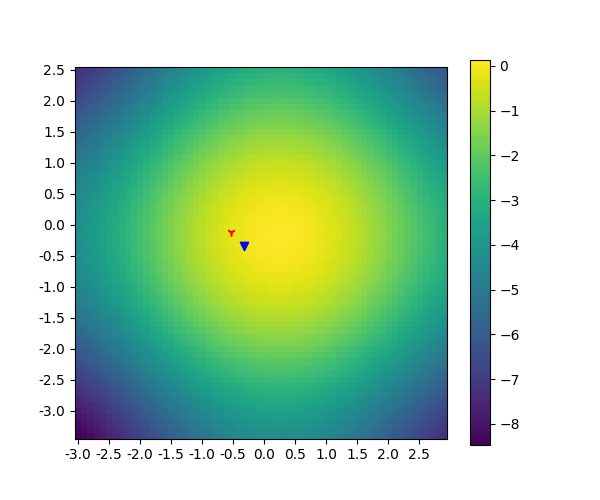
\includegraphics[width=60mm]{/Users/victor/Desktop/p7p_t049.png}}
\subfigure[Paso 100]{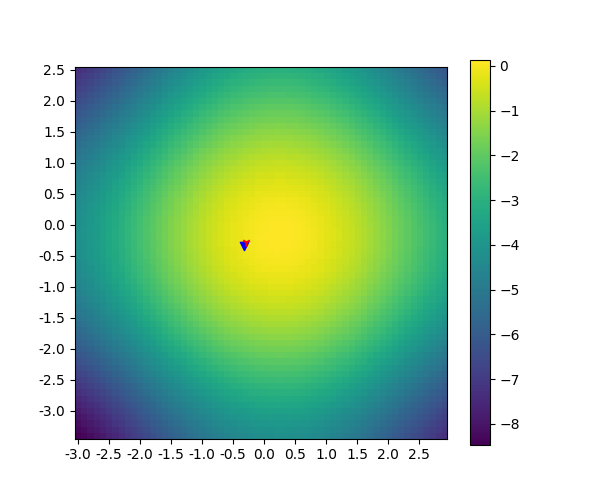
\includegraphics[width=60mm]{/Users/victor/Desktop/p7p_t099.png}}
\caption{B\'usqueda local simple.} 
\label{f1}
\end{figure}

Cómo se puede observar en la figura \ref{f1}, se tienen tres graficas en diferente tiempo. En color rojo se tiene la posición actual, mientras el mejor valor encontrado se encuentra en color azul.\\

Una vez completada la parte simple de esta tarea, se tomo como referencia \citep{DRA.Code} para en base a lo ya explicado realizar la tarea con las especificaciones finales.\\ 

Una vez finalizado el código se tiene un programa el cual cumple con las características pedidas.\\



\section{Conclusión}

A continuación, se podrán observar en la figura \ref{f2} los resultados del programa con las características pedidas.

\begin{figure}[H]
\centering
\subfigure[Paso 1]{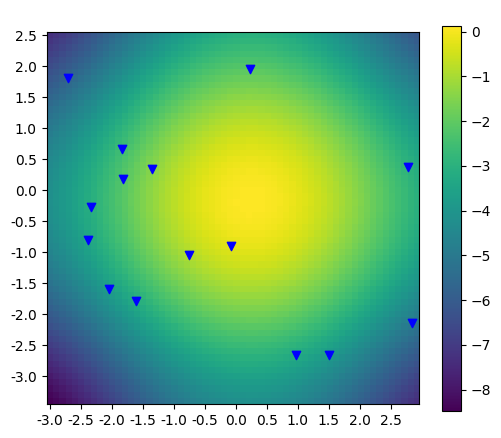
\includegraphics[width=60mm]{/Users/victor/Desktop/p7p_0.png}}
\subfigure[Paso 10]{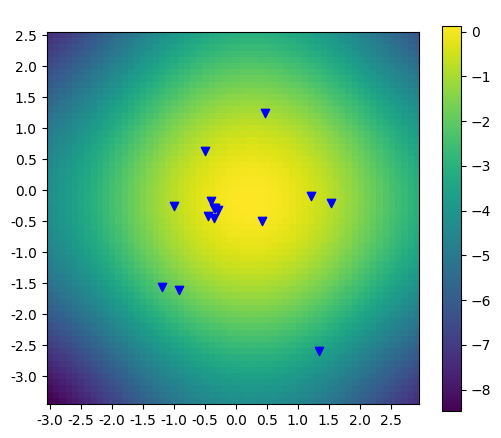
\includegraphics[width=60mm]{/Users/victor/Desktop/p7p_1.png}}
\subfigure[Paso 100]{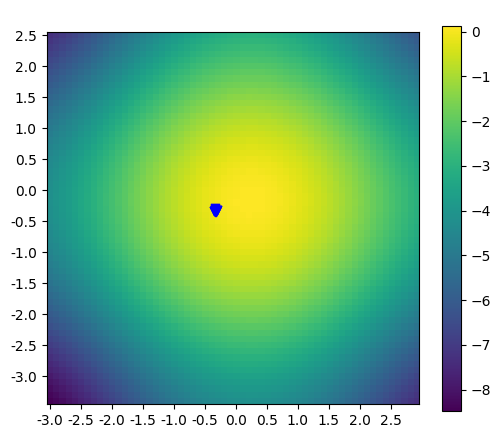
\includegraphics[width=60mm]{/Users/victor/Desktop/p7p_2.png}}
\subfigure[Paso 1000]{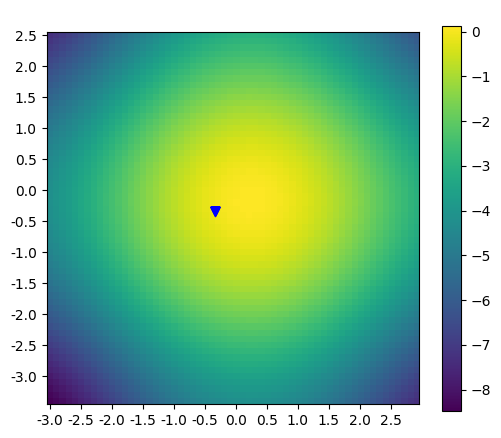
\includegraphics[width=60mm]{/Users/victor/Desktop/p7p_3.png}}
\caption{B\'usqueda local multiple.} 
\label{f2}
\end{figure}


Como conclusión, se puede observar en la  figura \ref{f2} como mientras mas pasos se tengan, mayor será la cantidad de puntos que encuentren el mayor local de la función. Sin embargo, se debe de tomar en cuenta el valor de $\Delta x$ y $\Delta y$ ya que dependiendo de este será la capacidad de encontrar el máximo o mínimo en la búsqueda local.

%-------------------------- Por si se rompe la URL --------------------------
\Urlmuskip=0mu plus 1mu\relax
%-------------------------- Por si se rompe la URL --------------------------
\bibliography{ref.Tarea7.bib}
\bibliographystyle{plainnat}

\end{document}